% CAP 6411 final report. Built on the official CVPR author kit
% (https://github.com/cvpr-org/author-kit, commit 1fd5709); see README.md to build.

\documentclass[10pt,twocolumn,letterpaper]{article}

% Course report: camera-ready layout (no line numbers, authors shown) with page numbers.
\usepackage[pagenumbers]{cvpr}

%% This file contains a number of tweaks that are typically applied to the main document.
%% They are not enabled by default, but can be enabled by uncommenting the relevant lines.


%%
%% Official support for 2-column teaser figure
%%
\usepackage{cuted} %< for strip environment

%%
%% For auto-referencing of figures (see fig/teaser.tex and \label{} therein)
%%
\usepackage{currfile} %< for \currfilebase macro

%%
%% caption and (global) spacing overrides
%%
\usepackage{caption} %< for "\captionof" commands (teaser)
% \setlength{\abovecaptionskip}{.5em} % space above caption
% \setlength{\belowcaptionskip}{1em} % space below caption

%%
%% Inline annotations; for predefined colors, refer to "dvipsnames" in the xcolor package:
%% https://tinyurl.com/overleaf-colors
%%
\newcommand{\red}[1]{{\color{red}#1}}
\newcommand{\todo}[1]{{\color{red}#1}}
\newcommand{\TODO}[1]{\textbf{\color{red}[TODO: #1]}}
%%
%% Disable for camera ready / submission by uncommenting these lines:
%%
% \renewcommand{\TODO}[1]{}
% \renewcommand{\todo}[1]{#1}

%%
%% Work harder in optimizing text layout. Typically shrinks text by 1/6 of page, enable
%% it at the very end of the writing process, when you are just above the page limit.
%%
% \usepackage{microtype}

%%
%% Fine-tune paragraph spacing.
%%
% \renewcommand{\paragraph}[1]{\vspace{.5em}\noindent\textbf{#1.}}

%%
%% Globally adjusts space between figure and caption.
%%
% \setlength{\abovecaptionskip}{.5em}

%%
%% Allows "the use of \paper to refer to the project name"
%% with automatic management of space at the end of the word.
%%
% \usepackage{xspace}
% \newcommand{\paper}{ProjectName\xspace}

%%
%% Commonly used math definitions.
%%
% \DeclareMathOperator*{\argmin}{arg\,min}
% \DeclareMathOperator*{\argmax}{arg\,max}

%%
%% Tighten underline.
%%
% \usepackage{soul}
% \setuldepth{foobar}

%%
%% Fix misplaced line numbers with lineno v5.7/v5.8 (Feb 2026, e.g. early TeX Live 2026 installs).
%% These versions write the column tag outside the column box, so line numbers end up on the
%% wrong side of the column. This backports the fix from lineno v5.9 and does nothing for other
%% lineno versions or in camera-ready mode. Updating TeX Live (tlmgr update --all) also fixes it.
%%
\makeatletter
\@ifpackageloaded{lineno}{\ifdefined\IfFormatAtLeastTF\IfFormatAtLeastTF{2025-06-01}{%
  \@ifpackagelater{lineno}{2026/03/08}{}{\@ifpackagelater{lineno}{2026/02/16}{%
    \RemoveFromHook{build/column/before}[lineno]%
    \AddToHook{build/column/after}{%
      \setbox\@outputbox\vbox to\ht\@outputbox{%
        \boxmaxdepth\@maxdepth
        \protected@write\@auxout{}{%
          \string\def\string\@LN@column{\if@firstcolumn1\else2\fi}}%
        \unvbox\@outputbox}}%
  }{}}}{}\fi}{}
\makeatother

\usepackage{booktabs}
\usepackage{tikz}
\usetikzlibrary{arrows.meta,positioning,fit,calc}
\usepackage{tcolorbox}
\tcbuselibrary{breakable}

% Section owners' notes: facts the repository already supports, to be turned into prose.
% Remove every notes box before submission.
\newtcolorbox{notes}[1]{breakable,colback=yellow!8,colframe=orange!70!black,boxrule=0.4pt,
  left=3pt,right=3pt,top=2pt,bottom=2pt,fonttitle=\footnotesize\bfseries,
  title={Notes for #1 (delete before submission)},fontupper=\footnotesize}

\definecolor{cvprblue}{rgb}{0.21,0.49,0.74}
\usepackage[pagebackref,breaklinks,colorlinks,allcolors=cvprblue]{hyperref}

\def\confName{CAP 6411}
\def\confYear{Fall 2026}

\title{When to Look: Change-Gated Invocation of a Compact\\Vision-Language Model for an Always-On Webcam Assistant}

\author{Alejandro \TODO{surname} \and Austin \TODO{surname} \and James \TODO{surname} \and Shawn \TODO{surname}\\
University of Central Florida\\
{\tt\small \TODO{emails}}}

\begin{document}
\maketitle
% Owner: James and Shawn (they coordinate the report, 4e plan, issue #25). Write last, about 150 words.
\begin{abstract}
\TODO{Abstract: James and Shawn, written last.}
\begin{notes}{James and Shawn}
\begin{itemize}\setlength\itemsep{0pt}
\item Problem: an always-on webcam assistant that asks a compact VLM about every frame wastes compute and battery while nothing happens.
\item Approach: a cheap frame-difference change gate decides when SmolVLM2-500M analyzes a frame; answers are schema-constrained and validated; a shared scene state turns answers into gesture onsets and offsets.
\item Task: fixed-camera \texttt{thumbs\_up} and \texttt{peace\_sign} recognition (master plan revision 9).
\item Headline functional check (Mac mini, 10 pilot clips): gated at 0.5\,s checks made 303 calls versus 1,348 for fixed 2\,s sampling and named 14 of 14 gestures versus 10 of 14 (Tab.~\ref{tab:pilot}, Figs.~\ref{fig:calls}--\ref{fig:timeline}).
\item Energy: state what was measured, per the option chosen in Sec.~\ref{sec:energy}.
\item Negative results are acceptable (course rubric): false gesture mentions on two clips (Sec.~\ref{sec:limitations}).
\end{itemize}
\end{notes}
\end{abstract}

% Owner: James and Shawn (4e plan). Austin and Alejandro review the system description.
\section{Introduction}
\label{sec:intro}
\TODO{Introduction prose: James and Shawn.}
\begin{notes}{James and Shawn}
\begin{itemize}\setlength\itemsep{0pt}
\item Primary research question (\texttt{docs/methodology.md}): can runtime scheduling reduce the energy of an always-on, on-device VLM assistant while keeping useful event quality and acceptable response delay?
\item Supplementary questions there: event-driven versus fixed-interval energy; quality and delay retained under selective calls; operating within an energy budget. The last one was not built (Sec.~\ref{sec:future}); say so here.
\item Framing from the methodology doc: compact VLMs make each call cheaper; this project asks whether a call is needed at all. Savings are an outcome to measure, not an assumption.
\item Contributions to list (check against what is in the final results): (1) a persistent local CPU inference stack with pinned model and runtime (1a); (2) qualified whole-laptop battery telemetry under WSL2 (1b); (3) a change gate, validated answer format and shared gesture event derivation (2a, 2c, 2b); (4) versioned file contracts and validators (2d); (5) the pilot gesture dataset (1e, 2e).
\item Platform: Ubuntu 22.04.5 under WSL2 on the team laptop, CPU only.
\end{itemize}
\end{notes}

% Owner: Shawn (methods and related work, docs/methodology.md "Related work and research framing").
% Every citation must come from arXiv or an official source; BibTeX lives in main.bib.
\section{Related Work}
\label{sec:related}
\TODO{Related Work prose: Shawn. The methodology doc's related-work section is the source draft.}
\begin{notes}{Shawn}
\begin{itemize}\setlength\itemsep{0pt}
\item \textbf{Compact VLMs.} SmolVLM~\cite{marafioti2025smolvlm} designs small VLMs for constrained devices (pixel shuffle to cut visual tokens; smallest 256M model under 1\,GB of GPU memory at inference). We run its SmolVLM2-500M video-instruct variant as a Q8\_0 GGUF in llama.cpp~\cite{llamacpp}. MobileVLM~\cite{chu2023mobilevlm} pairs 1.4B and 2.7B language models with an efficient projector and reports speed on a Snapdragon 888 CPU and a Jetson Orin. FastVLM~\cite{vasu2025fastvlm} attacks vision-encoder latency and visual token count with FastViTHD and reports a 3.2$\times$ faster time to first token in its LLaVA-1.5 setup.
\item Point to make: these reduce the cost of one call; our system decides whether a call happens, and holds the model fixed while comparing policies.
\item \textbf{Frame filtering for video queries.} NoScope~\cite{kang2017noscope} skips frames with cheap difference detectors and specialized models before running an expensive network. Our gate plays the same role in front of a VLM, with a persistence rule and a reference that moves only when a frame is sent.
\item \textbf{Adaptive frame selection.} AdaFrame~\cite{wu2019adaframe} learns which frames to look at for video recognition. Ours is a fixed rule with no training.
\item \textbf{Early exit and conditional computation.} BranchyNet~\cite{teerapittayanon2017branchynet} exits early from a network when confident; SkipNet~\cite{wang2018skipnet} learns to skip layers per input. Both save compute inside a model; our gate saves whole model calls.
\item The methodology doc also discusses VideoBrain and PolyThrottle; add BibTeX from arXiv or the publisher if they stay.
\end{itemize}
\end{notes}

% Owners: Alejandro drafted 3.1 to 3.5 (items 2a, 2b, 2c, 1d, 3c; app/, src/gates/, src/vlm/prompts.py).
% Austin owns 3.6 (inference and telemetry, items 1a and 1b; src/vlm/, src/energy/) and reviews
% the architecture as a whole (4e plan). Every number below is traced in a comment to its source.
\section{Method}
\label{sec:method}

% Pipeline figure (Alejandro). Stages match app/main.py, src/gates/change.py,
% src/vlm/prompts.py and app/state.py.
\begin{figure*}[t]
\centering
\resizebox{\textwidth}{!}{%
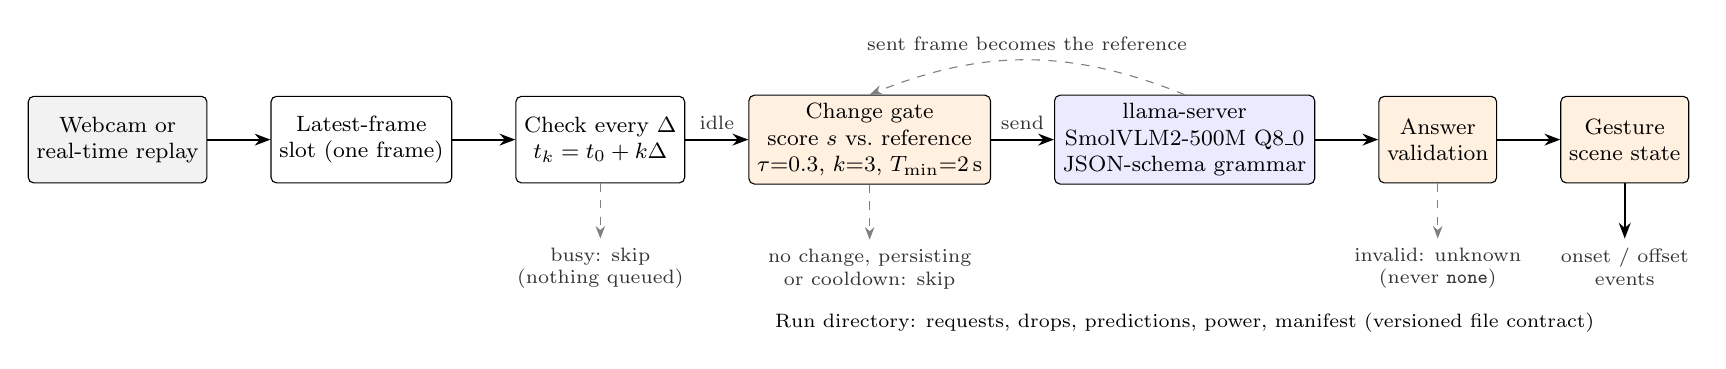
\begin{tikzpicture}[
  font=\footnotesize,
  box/.style={draw, rounded corners=2pt, align=center, minimum height=11mm, inner sep=3pt, fill=#1},
  box/.default=white,
  arr/.style={-{Stealth[length=2mm]}, thick},
  skip/.style={-{Stealth[length=1.6mm]}, gray, dashed},
  lab/.style={font=\scriptsize, gray!40!black, align=center},
  node distance=8mm
]
\node[box=gray!10] (cam) {Webcam or\\real-time replay};
\node[box, right=of cam] (slot) {Latest-frame\\slot (one frame)};
\node[box, right=of slot] (tick) {Check every $\Delta$\\$t_k=t_0+k\Delta$};
\node[box=orange!12, right=of tick] (gate) {Change gate\\score $s$ vs.\ reference\\$\tau{=}0.3$, $k{=}3$, $T_{\min}{=}2$\,s};
\node[box=blue!8, right=of gate] (vlm) {llama-server\\SmolVLM2-500M Q8\_0\\JSON-schema grammar};
\node[box=orange!12, right=of vlm] (val) {Answer\\validation};
\node[box=orange!12, right=of val] (scene) {Gesture\\scene state};

\draw[arr] (cam) -- (slot);
\draw[arr] (slot) -- (tick);
\draw[arr] (tick) -- node[lab, above]{idle} (gate);
\draw[arr] (gate) -- node[lab, above]{send} (vlm);
\draw[arr] (vlm) -- (val);
\draw[arr] (val) -- (scene);

% Skips and feedback.
\node[lab, below=7mm of tick] (busy) {busy: skip\\(nothing queued)};
\draw[skip] (tick) -- (busy);
\node[lab, below=7mm of gate] (gskip) {no change, persisting\\or cooldown: skip};
\draw[skip] (gate) -- (gskip);
\draw[skip] (vlm.north) to[bend right=22] node[lab, above]{sent frame becomes the reference} (gate.north);
\node[lab, below=7mm of val] (unk) {invalid: unknown\\(never \texttt{none})};
\draw[skip] (val) -- (unk);
\node[lab, below=7mm of scene] (ev) {onset / offset\\events};
\draw[arr] (scene) -- (ev);

% Logs.
\node[lab, below=15mm of vlm, text=black] (logs) {Run directory: requests, drops, predictions, power, manifest (versioned file contract)};
\end{tikzpicture}}
\caption{The assistant's pipeline. Orange stages are the parts described in Secs.~\ref{sec:gate} to \ref{sec:scene}. The fixed-interval baseline is the same pipeline with the gate removed, so it sends every check at which no request is in flight. Every skipped check is logged with its reason.}
\label{fig:pipeline}
\end{figure*}


The assistant watches one camera and reports when a person starts or stops showing a thumbs-up or a peace sign.
Figure~\ref{fig:pipeline} shows the pipeline.
A capture thread keeps only the newest frame, a scheduler decides at regular checks whether that frame goes to the vision-language model (VLM), the model's answer is constrained to a fixed format and validated, and a scene state turns the stream of validated answers into gesture events.
The fixed-interval baseline and the gated policy share every stage except the gate, so any difference between them comes from which frames are sent.

\subsection{Capture and scheduling}
\label{sec:schedule}
% Source: app/main.py module docstring and _main_loop.
Capture runs on its own thread and overwrites a single slot with each new frame, so slow inference never stalls capture and no backlog of stale frames builds up.
The scheduler wakes at checks $t_k = t_0 + k\Delta$ on the monotonic clock, so checks do not drift when one runs late.
At each check it takes the newest frame and applies three rules in order.
If a request is still in flight, the check is skipped and logged as busy; nothing is queued.
If an earlier request timed out, the scheduler waits until the server reports no busy slot before sending again.
Otherwise the frame is sent under the fixed-interval policy, or passed to the change gate under the gated policy.
At most one request is in flight at any time.
Every skipped check is written to the run's drop log with its reason, so the logs account for every check.

\subsection{Change gate}
\label{sec:gate}
% Source: src/gates/change.py (GateConfig defaults and ChangeGate.decide/acknowledge).
The gate compares the candidate frame with a \emph{reference}: the last frame actually sent to the VLM.
Comparing against the last sent frame, instead of the previous frame, lets a change that builds up slowly keep growing until it triggers.

\paragraph{Change score.}
Each frame is converted to grayscale, resized to $160\times120$, blurred with a $5\times5$ Gaussian kernel, and its mean brightness is subtracted, so a uniform lighting shift does not count as change.
For a preprocessed frame $f$ and reference $r$, a pixel $p$ is changed when $|f(p)-r(p)| > \delta$, with $\delta=25$ on the 0 to 255 brightness scale.
The image is divided into a $4\times4$ grid of cells $C_j$, and the score is the changed fraction of the most-changed cell,
\begin{equation}
  s = \max_j \frac{1}{|C_j|}\sum_{p\in C_j} \mathbb{1}\big[\,|f(p)-r(p)|>\delta\,\big].
  \label{eq:score}
\end{equation}
Taking the maximum over cells keeps a hand raised in one part of the frame from being diluted by the static remainder.
The whole-frame changed fraction is logged beside $s$ for diagnosis.

\paragraph{Decision.}
A change starts when $s \ge \tau$ and must stay above $\tau$ for $k$ consecutive checks before it triggers a call; a score below $\tau$ resets the count.
After a trigger, further triggers are held back for a cooldown $T_{\min}$.
In order, the gate (1) triggers when it has no reference yet, (2) skips when $s<\tau$, (3) skips while the change has lasted fewer than $k$ checks, (4) skips within $T_{\min}$ of the last trigger, and (5) otherwise triggers.
When a triggered frame is sent, it becomes the new reference, the cooldown clock restarts and the persistence count resets.
The gate is consulted only when no request is in flight, so every trigger is sent, and a busy check neither advances nor resets the count.
The implementation also supports a periodic forced refresh and a lower release threshold (hysteresis); both are off by default.

\paragraph{Settings.}
% Source: GateConfig defaults; README "Choosing the gate settings" for the tuning evidence.
We use $\tau=0.3$, $k=3$ and $T_{\min}=2$\,s with checks every $\Delta=0.5$\,s, so a change must be present at three checks spanning 1\,s before it is sent.
These values were chosen on development clips.
On \texttt{real\_thumbs\_1}, ordinary movement scores 0.02 (median) to 0.40 (99th percentile), while a thumbs-up peaks at 0.68 to 0.75.
An earlier setting ($\tau=0.05$ without persistence) fired on head movement and made more calls than fixed 2\,s sampling.
With $\tau=0.3$ and $k=3$, a replay that models each call as 2.5\,s of busy time caught both gestures on \texttt{real\_thumbs\_1} with 27 calls against 147 for fixed 2\,s sampling, 82\% fewer.
A threshold of 0.4 cut calls further but left less margin under the gesture scores, and hysteresis only added calls on these clips.
Because $k$ counts checks, these settings are tied to $\Delta=0.5$\,s and must be retuned for another check interval.

\subsection{Validated answer format}
\label{sec:answers}
% Source: src/vlm/prompts.py (GESTURE_PROMPT, GESTURE_SCHEMA, parse_gesture_answer, ANSWER_ERRORS);
% configs/inference.json (max_output_tokens 64).
Every request asks the same question about one frame: \emph{``Describe what the person's hands are doing in a few words, then say whether the person is making a thumbs up, a peace sign, or neither (none).''}
The request carries a JSON schema that llama-server compiles into a decoding grammar, so a compliant server can only return an object with two fields in a fixed order: \texttt{hands}, a free description of at most 80 characters, then \texttt{gesture}, one of \texttt{thumbs\_up}, \texttt{peace\_sign} or \texttt{none}.
The \texttt{hands} field comes first because SmolVLM2 asked for the gesture alone answered \texttt{thumbs\_up} on every frame; writing a short description first gives the model a step in which to look before it commits to a label.
Only \texttt{gesture} is used as the observation.

The application validates every answer exactly, without normalizing or guessing, because the constraint can fail: a server may ignore the schema, or the 64-token output bound may cut an answer short.
An answer that fails validation is recorded with one of seven reasons (truncated, not JSON, not an object, missing field, unexpected fields, non-text description, gesture outside the vocabulary) and is treated as \emph{unknown}.
An unknown answer is never read as \texttt{none}: \texttt{none} is a positive statement that neither gesture is visible, while an unknown answer carries no information.
Transport status (whether the server answered) is logged separately from answer validity.

\subsection{Gesture scene state}
\label{sec:scene}
% Source: app/state.py (GestureScene.update, Evidence.available_source_time_s).
The scene state holds one confirmed gesture, starting at \texttt{none}, and updates once per request.
A validated answer equal to the confirmed gesture changes nothing, so a held gesture is reported once.
A different validated answer confirms a change after $c$ consecutive answers agree ($c=1$ by default): leaving a gesture emits an \emph{offset}, entering one emits an \emph{onset}, and a direct switch between the two gestures emits both from the same answer.
Returning to \texttt{none} rearms the state, so the same gesture shown again is a new onset.
Unknown answers (failed requests or invalid answers) change nothing: the confirmed gesture stays, and a change awaiting confirmation neither advances nor resets.
The state also counts unknown answers since the last valid one, which the display shows as staleness.

Each event keeps the request it came from, with the frame's source time and the time the answer became available.
The event time used for scoring is the availability time mapped onto the source timeline,
$t_{\text{avail}} = t_{\text{src}} + (t_{\text{resp}} - t_{\text{cap}})$,
where $t_{\text{src}}$ is the frame's media time, $t_{\text{cap}}$ its host capture time and $t_{\text{resp}}$ the host time the answer arrived.
Response delay therefore includes the time the frame waited to be sent and the inference time, and does not credit an answer with the moment its frame was captured.
Both policies feed the same scene state, so fixed and gated runs share one event derivation.

\subsection{Run records}
\label{sec:records}
% Source: app/main.py module docstring; docs/data-contracts.md (item 2d); src/contracts/.
Each run writes a new directory with a request log (one line per call, with frame identity, source time, request and response times, transport status, validated gesture or answer error), a drop log (every skipped check and every frame the source dropped, with its reason and gate score), the derived gesture events, power samples and a manifest of the configuration and platform.
The formats follow the project's versioned file contract, and a validator checks every run directory, so the evaluation tools read files and never application internals.
Unavailable power, token or timing values are recorded as missing, never as zero.

\subsection{Inference and telemetry}
\label{sec:inference}
% Owner: Austin (items 1a, 1b). Alejandro: facts below are from configs/inference.json and
% docs/1b-battery-qualification.md; Austin turns them into prose and checks them.
\TODO{Inference and telemetry prose: Austin.}
\begin{notes}{Austin}
\begin{itemize}\setlength\itemsep{0pt}
\item Model: SmolVLM2-500M-Video-Instruct, Q8\_0 GGUF with its Q8\_0 projector (\texttt{ggml-org/SmolVLM2-500M-Video-Instruct-GGUF}, pinned revision and SHA-256 in \texttt{configs/inference.json}).
\item Runtime: one persistent llama-server from llama.cpp~\cite{llamacpp} revision 620d222, CPU only, 4 threads, context 4096, output bound 64 tokens, 120\,s read timeout, localhost port 8080.
\item Client: \texttt{src/vlm/client.py}; failed requests are logged, never retried silently. Frames sent as JPEG at quality 85 (\texttt{app/main.py}).
\item Team-laptop smoke check (1a, \texttt{docs/validation-1a-1b.md}): mean request latency 2.48\,s under WSL2 on CPU.
\item Telemetry (1b): whole-laptop battery energy from Windows \texttt{BatteryReport} read from WSL2; WSL sysfs scale is unqualified and RAPL is absent, so package energy is unavailable. Details in Sec.~\ref{sec:setup}.
\end{itemize}
\end{notes}

% Owner: Shawn (protocol, benchmarks; items 1f, 2f, 3f) and James (data; items 1e, 2e).
\section{Experimental Setup}
\label{sec:setup}
\TODO{Experimental Setup prose: Shawn and James.}
\begin{notes}{Shawn and James}
\begin{itemize}\setlength\itemsep{0pt}
\item \textbf{Data} (\texttt{data/README.md}, \texttt{data/annotations/pilot.csv}): James's session S1, fixed camera. \texttt{control} (idle), \texttt{recording\_1..4} ($\sim$10\,s, one gesture each), \texttt{thumbs\_mov\_1..6} (10 to 30\,min, mostly idle, two thumbs-ups each). The CSV holds 16 events (14 thumbs-up, 2 peace sign) in 10 videos; all one group, splits blank; pilot data only, no held-out split. Note \texttt{thumbs\_mov\_1/2} are the clips called \texttt{real\_thumbs\_1/2} elsewhere.
\item \textbf{Event rule:} a shape held at least 0.5\,s; ends when the hand drops or the shape breaks; repeating after a drop is a new event; other hand motion is negative.
\item \textbf{Policies:} fixed interval ($\Delta=2$\,s, every free check sent) and gated ($\Delta=0.5$\,s checks, gate defaults of Sec.~\ref{sec:gate}). The planned budget-aware policy was not built.
\item \textbf{Metrics:} a window is \emph{caught} when a call lands inside it and \emph{named} when an answer inside it gives that window's gesture; a \emph{false mention} is a gesture answer outside every window; delay is onset to the first naming answer's availability time. Scored by \texttt{scripts/gate\_check.py} at $\pm1$\,s tolerance (annotations run about 1\,s off). The planned one-to-one event matcher (3d, 3e) was not built; say so.
\item \textbf{Platforms:} team laptop, Ubuntu 22.04.5 under WSL2, CPU (the only platform for energy). Functional checks ran on a Mac mini (Apple silicon, CPU build of the same pinned llama.cpp and model) and carry no energy claims.
\item \textbf{Energy source} (\texttt{docs/1b-battery-qualification.md}): Windows \texttt{BatteryReport} via PowerShell from WSL2, on battery only. Qualification run 270.6\,s: 3.089\,Wh drop; median reported power 41.2\,W idle, 37.4\,W under a 4-worker CPU load, 37.6\,W recovery; updates every 30 to 40\,s in steps of about 0.39\,Wh. It cannot attribute energy to single calls, and it did not show the CPU load.
\item \textbf{Reproduction:} README commands; each run writes a new directory checked by \texttt{uv run contracts-check RUN\_DIR}.
\end{itemize}
\end{notes}

% Owners: Shawn (analysis, 3g, 4d) and James (event scoring, 4a) for the section as a whole.
% Alejandro drafted 5.1 (functional check) and the two energy options in 5.2; he picks one.
\section{Results}
\label{sec:results}

\subsection{Functional check on the pilot clips}
\label{sec:pilot}
% Source: docs/report/data/pilot-2026-11-18.csv (rows whose windows_from equals clip).
% Runs: Mac mini, one llama-server, real-time replays one at a time, 18 Nov 2026,
% fixed --interval-s 2, gated --policy gated --interval-s 0.5, gate defaults.

\begin{table}[t]
\centering
\footnotesize
\setlength{\tabcolsep}{3.5pt}
\resizebox{\columnwidth}{!}{%
\begin{tabular}{@{}lc rr rr rr@{}}
\toprule
 & & \multicolumn{2}{c}{Calls} & \multicolumn{2}{c}{Named} & \multicolumn{2}{c}{False mentions} \\
\cmidrule(lr){3-4}\cmidrule(lr){5-6}\cmidrule(l){7-8}
Clip & Win. & Fixed & Gated & Fixed & Gated & Fixed & Gated \\
\midrule
recording\_1\_thumbs & 1 & 4 & 3 & 1 & 1 & 0/2 & 0/2 \\
recording\_2\_thumbs & 1 & 3 & 3 & 0 & 1 & 0/2 & 0/2 \\
recording\_3\_peace  & 1 & 3 & 3 & 0 & 1 & 0/1 & 0/2 \\
recording\_4\_peace  & 1 & 3 & 3 & 1 & 1 & 0/2 & 0/2 \\
control             & 0 & 3 & 1 & -- & -- & 0/3 & 0/1 \\
real\_thumbs\_1     & 2 & 147 & 25 & 2 & 2 & 1/143 & 0/21 \\
real\_thumbs\_2     & 2 & 133 & 26 & 1 & 1 & 7/128 & 9/24 \\
thumbs\_mov\_3      & 2 & 336 & 106 & 2 & 2 & 91/330 & 52/101 \\
thumbs\_mov\_4      & 2 & 363 & 39 & 1 & 2 & 7/361 & 3/36 \\
thumbs\_mov\_5      & 2 & 353 & 94 & 1 & 2 & 140/350 & 49/90 \\
\midrule
All 10 clips        & 14 & 1,348 & 303 & 9 & 13 & 246/1,322 & 113/281 \\
\bottomrule
\end{tabular}}
\caption{\textbf{Mac mini, functional check} (no energy measured). Fixed sampling checks every 2\,s; the gated policy checks every 0.5\,s with $\tau{=}0.3$, $k{=}3$, $T_{\min}{=}2$\,s. \emph{Win.}: annotated gesture windows. \emph{Named}: windows in which an answer gave the window's gesture. \emph{False mentions}: gesture answers among the calls made outside every window. Scored at $\pm1$\,s.}
\label{tab:pilot}
\end{table}

Table~\ref{tab:pilot} compares the two policies on the ten pilot clips, about 90 minutes of video replayed in real time on a Mac mini.
These runs check that the pipeline behaves as designed; they are not energy results, and the clips include those used to choose the gate settings.
Over all clips the gated policy made 303 calls against 1,348 for fixed sampling, 78\% fewer, and named 13 of the 14 gesture windows against 9.
% 303/1348 = 0.225. Named: windows_named column.
Every one of the 1,651 answers validated against the schema.
% answers_invalid is 0 in every row; 1,348 + 303 = 1,651.

Fixed sampling at 2\,s did not achieve a 2\,s rate.
The median call took 2.5\,s, longer than the interval, so nearly every other check found a request in flight: the fixed runs skipped 1,342 checks as busy against 1,348 calls, which spaces calls about 4\,s apart.
% busy_skips column, fixed rows: 1,342; median_call_s about 2.5 in every row.
Both policies placed at least one call in every window except one; the fixed policy's five misses are windows where its few calls returned \texttt{none} or the wrong gesture.
% windows_caught: fixed 14 of 14, gated 13 of 14; wrong_gesture_in_window: fixed 3.
The gated policy waits for a change to persist for 1\,s and then sends a frame in which the gesture has settled, which is consistent with it naming more windows with fewer calls.
Its one miss is the first window of \texttt{real\_thumbs\_2}, where the annotation appears to be placed about a minute early; neither policy names it.
\TODO{Alejandro: keep or drop the annotation remark; with that window moved one minute later both policies catch it (gated 14 of 14, fixed 10 of 14), see the CSV row real\_thumbs\_2\_minutefix.}

For windows that were named, the median delay from gesture onset to the naming answer's availability was 4.06\,s for the gated policy (13 windows) and 4.61\,s for fixed sampling (9 windows).
% Pooled delays_s column over the ten clips.
Most of the gated delay is the 1\,s persistence wait and one call of about 2.5\,s; the gate can start counting while the hand is still rising, before the annotated onset, so some delays are shorter than that sum.

The gated policy did not reduce false mentions in proportion to calls.
It made 113 false mentions in 281 calls outside gesture windows (40\%) against 246 in 1,322 for fixed sampling (19\%).
Gated calls happen when something moves, and movement is when the model is most easily misled, so the gate concentrates calls on the frames the model finds hardest.
Most false mentions come from two clips, \texttt{thumbs\_mov\_3} and \texttt{thumbs\_mov\_5} (Sec.~\ref{sec:limitations}); on the other eight clips they total 15 for fixed and 12 for gated.
% Fixed: 1+7+7 = 15; gated: 9+3 = 12 (false_mentions_outside column).
Each false mention that differs from the confirmed gesture becomes an onset, so the scene state wrote 167 onsets in the fixed runs and 85 in the gated runs, against 14 annotated gestures.
% app_onsets column.

\TODO{James and Shawn: held-out event quality (4a) if any is run; otherwise state that the pilot clips are the only quality evidence.}

\subsection{Energy}
\label{sec:energy}
% Alejandro picks option A or B; delete the other. Owner of the final text: Shawn (3g, 4d) with Austin.
\begin{tcolorbox}[colback=red!4,colframe=red!60!black,boxrule=0.5pt,fonttitle=\footnotesize\bfseries,title={Placeholder: Alejandro picks option A or B and deletes the other},fontupper=\small]
\textbf{Option A: team-laptop battery runs.}
We replayed \TODO{clips} on the team laptop under WSL2 on battery power, once per policy and \TODO{N} times each, reading whole-laptop energy from the qualified Windows battery report.
Fixed sampling used \TODO{X}\,Wh over \TODO{T}\,min and the gated policy \TODO{Y}\,Wh, a difference of \TODO{D}\% (\TODO{spread across repeats}).
An idle run with the model loaded and no calls used \TODO{I}\,Wh over the same time, so the incremental energy of inference was \TODO{X$-$I} and \TODO{Y$-$I}\,Wh.
These are whole-laptop figures; package energy is unavailable under WSL2.

\medskip
\textbf{Option B: estimate from call counts (energy not measured end to end).}
We did not measure either policy's energy on the team laptop.
The qualified battery source reports whole-laptop energy in steps of about 0.39\,Wh every 30 to 40\,s, which cannot resolve single calls, and in its qualification run it reported 41.2\,W idle and 37.4\,W under a four-worker CPU load, so it did not register a CPU load of that size.
We therefore estimate from call counts and label the result as an estimate.
On the pilot replays the gated policy made 303 calls against 1,348.
At the median call time of 2.5\,s, the model was busy for about 760\,s under the gated policy and 3,370\,s under fixed sampling, out of about 5,380\,s of video.
At the laptop's reported 41.2\,W idle draw, the whole session costs about 62\,Wh under either policy, so the saving is the incremental inference power $\Delta P$ times the 2,610\,s of busy time avoided: about 0.73\,Wh for each watt of $\Delta P$.
We did not measure $\Delta P$, so this bounds the saving by a quantity we could not observe; the call reduction itself (78\%) is the measured result.
% 303*2.5 = 757.5 s; 1348*2.5 = 3370 s; replay length = (1348+1342)*2 s = 5380 s;
% 41.2 W * 5380 s = 61.6 Wh; (3370-757.5) s = 2612.5 s = 0.726 h. Call time is the Mac mini's;
% the team laptop's 1a smoke check measured a 2.48 s mean, close to it.
\end{tcolorbox}

% Owners: James and Shawn (4e plan). Alejandro drafted the false-mention and gate paragraphs.
\section{Limitations}
\label{sec:limitations}

\paragraph{False gesture mentions.}
% Source: docs/report/data/pilot-2026-11-18.csv, rows thumbs_mov_3 and thumbs_mov_5
% (false_mentions_outside, answers_thumbs_up, answers_peace_sign, outside_calls).
On two long clips the model often named a gesture that was not there.
On \texttt{thumbs\_mov\_3} it did so in 91 of 330 calls outside gesture windows under fixed sampling and 52 of 101 under the gated policy; on \texttt{thumbs\_mov\_5}, in 140 of 350 and 49 of 90.
On \texttt{thumbs\_mov\_5} with fixed sampling it answered \texttt{peace\_sign} 106 times, though the clip contains only thumbs-ups.
These two clips account for 231 of the 246 fixed false mentions and 101 of the 113 gated ones.
The scene state cannot easily filter them at our call rates: under fixed sampling calls arrive about 4\,s apart, so requiring two agreeing answers before an onset would add about 4\,s of delay and drop any gesture held for less than two calls.
We kept SmolVLM2-500M for every result; whether a larger model reduces false mentions at acceptable latency and energy is untested.

\paragraph{Gate.}
The gate settings were chosen on clips that also appear in Table~\ref{tab:pilot}, so the table is not a held-out estimate.
The gate responds to any localized change that persists, so a person who moves steadily in one region sends calls as readily as one who gestures, and a switch from one gesture to the other in the same place changes few pixels and may not trigger.
Its persistence count is defined in checks, so its timing depends on the check interval.

\TODO{James and Shawn: data limitations (one session, one person, 16 events, no grouped split, annotation offset of about 1\,s); Mac mini versus team laptop; energy source granularity; scorer is window-based (no one-to-one matcher).}

% Owner: whole team. Alejandro drafted the controller paragraph.
\section{Future Work}
\label{sec:future}

\paragraph{Budget-aware controller.}
The plan included an energy-budget controller (items 3a and 3c) that would admit gate triggers only while the measured energy stayed within an allowance, and an application mode running under it.
Neither was built.
The battery source's 30 to 40\,s update interval makes per-call admission impractical, so a controller would need either a finer power source or a model of per-call cost calibrated against longer battery windows.

\TODO{Team: other future work, for example held-out grouped evaluation, a one-to-one event matcher, larger or different compact VLMs for false mentions, repeated battery trials, and a learned gate.}

% Owner: whole team; Alejandro decides the final wording. Required by the course.
\section*{Contribution Statement}
\TODO{Team to agree. Draft from repository ownership (AGENTS.md), to be confirmed by each member:}
\begin{notes}{the team}
\begin{itemize}\setlength\itemsep{0pt}
\item \textbf{Alejandro:} capture and replay (1c), fixed-interval application (1d), change gate (2a), validated answer format (2c), gesture scene state (2b); report Secs.~\ref{sec:schedule} to \ref{sec:records}, \ref{sec:pilot}.
\item \textbf{Austin:} persistent local inference (1a), battery telemetry and qualification (1b), file contracts (2d, with James); architecture review.
\item \textbf{James:} pilot gesture dataset and annotations (1e, 2e); event scoring; report data sections.
\item \textbf{Shawn:} methodology and measurement protocol (1f), benchmark configurations; report analysis sections.
\end{itemize}
\end{notes}

% Owner: whole team. Required by the course. Placeholder until the team agrees on the wording.
\section*{Generative AI Disclosure}
\TODO{Placeholder for the team to agree on: which generative AI tools were used, for what (code, writing, figures), and how their output was checked.}

{
    \small
    \bibliographystyle{ieeenat_fullname}
    \bibliography{main}
}
\end{document}
